\section{Keplerian Orbital Elements}
%%%%%%%%%%%%%%%%%%%%%%%%%%%%%%%%%%%%%%%%%%%%%%%%%%%%%%%%%%%%%%%%%%%%
\begin{frame}
    \frametitle{Phase 1.3: Orbital Elements to Orbital State Vectors}
    \begin{itemize}
        \item For our n-body simulation, we need the two Cartesian vectors for each body: the position vector $\vec{r}$ and the velocity vector $\vec{v}$. 
        \item They are also called \textit{orbital state vectors}.
        \vspace*{1em}
        \item In astronomy the Kepler orbit is used more often to describe the mechanics of a celestial body.
        \item They are also called Keplerian \textit{orbital elements}.
    \end{itemize}
    \pause
    \vfill
    \itFollows{Since the data is given using the orbital elements, we must convert them to their respective orbital state vectors before we can use them in our simulation.}
\end{frame}
%%%%%%%%%%%%%%%%%%%%%%%%%%%%%%%%%%%%%%%%%%%%%%%%%%%%%%%%%%%%%%%%%%%%

\subsection{Definition}
%%%%%%%%%%%%%%%%%%%%%%%%%%%%%%%%%%%%%%%%%%%%%%%%%%%%%%%%%%%%%%%%%%%%
\begin{frame}
    \frametitle{Orbital Elements - Visualization: Shape and Size of the Ellipsis}
    \begin{center}
        \begin{tikzpicture}
\begin{scope}
    \shade[ball color = gray!40, opacity = 0.8] (0,0) circle (.2cm);
    \visible<2->{
        \draw (0, 0) circle (2cm);
        \node at (0, -2.5) {$e = 0$};
    };
    \visible<3->{
        \draw[dashed] (-2, 0) -- (0, 0);
        \draw[dashed] (0, 2) -- (0, -2);
        \draw[red] (0, 0) -- node[below=5pt] {$a$} ++(2, 0);
        \fill (0, 0) circle (.05cm);
    };
\end{scope}
\begin{scope}[shift={(6,0)}]
    \shade[ball color = gray!40, opacity = 0.8] (-.25,0) circle (.2cm);
    \visible<2->{
        \draw (1, 0) ellipse (2cm and 1.5cm);
        \node at (1, -2.5) {$e = \num{0.66}$};
    };
    \visible<3->{
        \draw[dashed] (-1, 0) -- (1, 0);
        \draw[dashed] (1, 1.5) -- (1, -1.5);
        \draw[red] (1, 0) -- node[below=5pt] {$a$} ++(2, 0);
        \fill (1, 0) circle (.05cm);
    };
\end{scope}
        \end{tikzpicture}
    \end{center}
    \begin{description}
        \setlength\itemsep{.5em}
        \item<2->[eccentricity $e$]\hfill\\\hspace*{-2cm} shape of the ellipsis (elongation compared to a circle)
        \item<3->[{semi-major axis $a\ [\si{\au}]$}]\hfill\\\hspace*{-2cm} one-half of the largest diameter
    \end{description}
\end{frame}
%%%%%%%%%%%%%%%%%%%%%%%%%%%%%%%%%%%%%%%%%%%%%%%%%%%%%%%%%%%%%%%%%%%%

%%%%%%%%%%%%%%%%%%%%%%%%%%%%%%%%%%%%%%%%%%%%%%%%%%%%%%%%%%%%%%%%%%%%
\begin{frame}[t]
    \frametitle{Orbital Elements - Visualization}
    \vspace*{-.9em}
    \begin{center}
        \begin{tikzpicture}[scale=1.1]
% reference plane
\draw[fill, color=gray!20] (-4, -1.5) -- (5.8, -1.5) -- (5, 1.5) -- (-4.8, 1.5) -- cycle;

% reference direction
\draw[color=gray!90, ->] (0, 0) -- (4, 0);
\node at (4.2, -.2) {\Aries};

\visible<6-|handout:6>{
    % argument of periapsis
    \draw[dashed, ForestGreen] (0, 0) -- (2.98, 1.98);
    \node (ap1) at (.12, -.4) {};
    \node (ap2) at (.925, .6) {};
    \draw[thick, ForestGreen, ->] (ap1.center) to[bend right=40, in=260] (ap2.center);
    \node[ForestGreen] at (.8, .25) {$\omega$};
}

\visible<7-|handout:7->{
    % true/mean anomaly
    \draw[dashed, red] (0, 0) -- (1.8, 2.2);
    \node (tma1) at (1.875, 1.25) {};
    \node (tma2) at (1.25, 1.525) {};
    \draw[thick, red, ->] (tma1.center) to[bend right=40, out=310] (tma2.center);
    \node[red] at (1.45, 1.275) {$\nu$};
}

\visible<2-|handout:2->{
    % orbit
    \draw[thick, rotate=30, opacity=0.75] (0.0, 0.0) ellipse (3.61cm and 1.5cm);
    \fill[color=gray!20, opacity=0.75] (-.35, 1.5) rectangle (-4, -1.5);
    \fill[white, opacity=0.6] (-4, -1.5) rectangle (.4, -2.5);
    % orbital body
    \shade[ball color=red!40] (1.8, 2.2) circle (.15cm);
    \node (obd1) at (1.8 + .45, 2.35) {};
    \node (obd2) at (1.8 - .45, 2.25) {};
    \draw[->] (obd1) to[bend right=20] (obd2);
}

\visible<3-|handout:3->{
    % inclination
    \node (i1) at (1.4, -1.5) {};
    \node (i2) at (1.3, -0.95) {};
    \draw[thick, blue, ->] (i1.center) to[bend right=40] (i2.center);
    \node[blue] (i) at (1.15, -1.275) {\bfseries $i$};
}

\visible<4-|handout:4->{
    % ascending node 
    \draw[dotted, color=gray!40] (.4, -1.5) -- (-.4, 1.5);
    \fill (.4, -1.5) circle (.05cm);
    \node at (.4, -1.85) {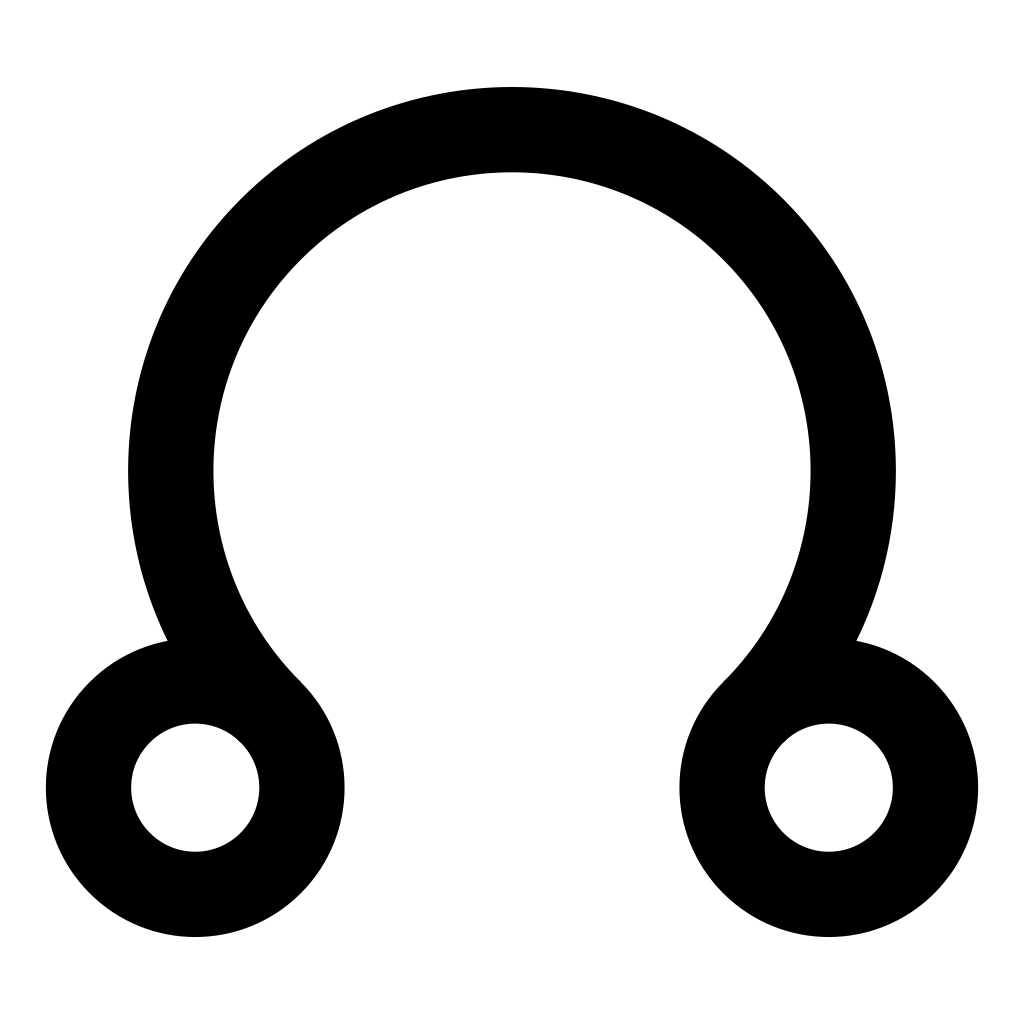
\includegraphics[width=.3cm]{figures/ascending_node}};
}
\visible<5-|handout:5->{
    % longitude of the ascending node
    \node (lan1) at (.6, 0) {};
    \node (lan2) at (.1, -.6) {};
    \draw[thick, orange, ->] (.45, 0) arc[start angle=0, end angle=280, x radius=.45, y radius=.25];
    \node[orange] at (-.7, 0) {$\Omega$};
}

% central body
\shade[ball color=gray!40] (0, 0) circle (.2cm);
\draw[fill, color=gray!20, opacity=0.75] (-0.2, -0.01) rectangle (0.2, -0.2);
        \end{tikzpicture}
    \end{center}
    \vspace*{.15em}
    
    \begin{tikzpicture}[overlay]
\only<1|handout:1>{
    \node[minimum size=\textwidth, align=left, anchor=west] at (-2.4, 0) {%
    reference direction \Aries:\\
    for heliocentric orbits also known as \enquote{First Point of Aries}};
}
\only<3|handout:3>{
    \node[minimum size=\textwidth, align=left, anchor=west] at (-.3, 0) {%
    \begin{varwidth}{\linewidth}
        \begin{description}
            \item[{inclination $i\ [\si{rad}]$}]\hfill\\\hspace*{-2cm} 
            vertical tilt of the ellipsis with respect to the reference plane, e.g.:\\\hspace*{-1cm}
            \begin{tabular}{r@{\hspace{3pt}}c@{\hspace{3pt}}rl}
                $\SI{0}{\radian}$ & $=$ & $\SI{0}{\degree}$ & orbital plane same as reference plane \\
                $\SI{1.5708}{\radian}$ & $=$ & $\SI{90}{\degree}$ & orbital plane perpendicular to reference plane
            \end{tabular}
        \end{description}
    \end{varwidth}};
}
\only<4|handout:4>{
    \node[minimum size=\textwidth, align=left, anchor=west] at (-1.3, 0) {%
    ascending node 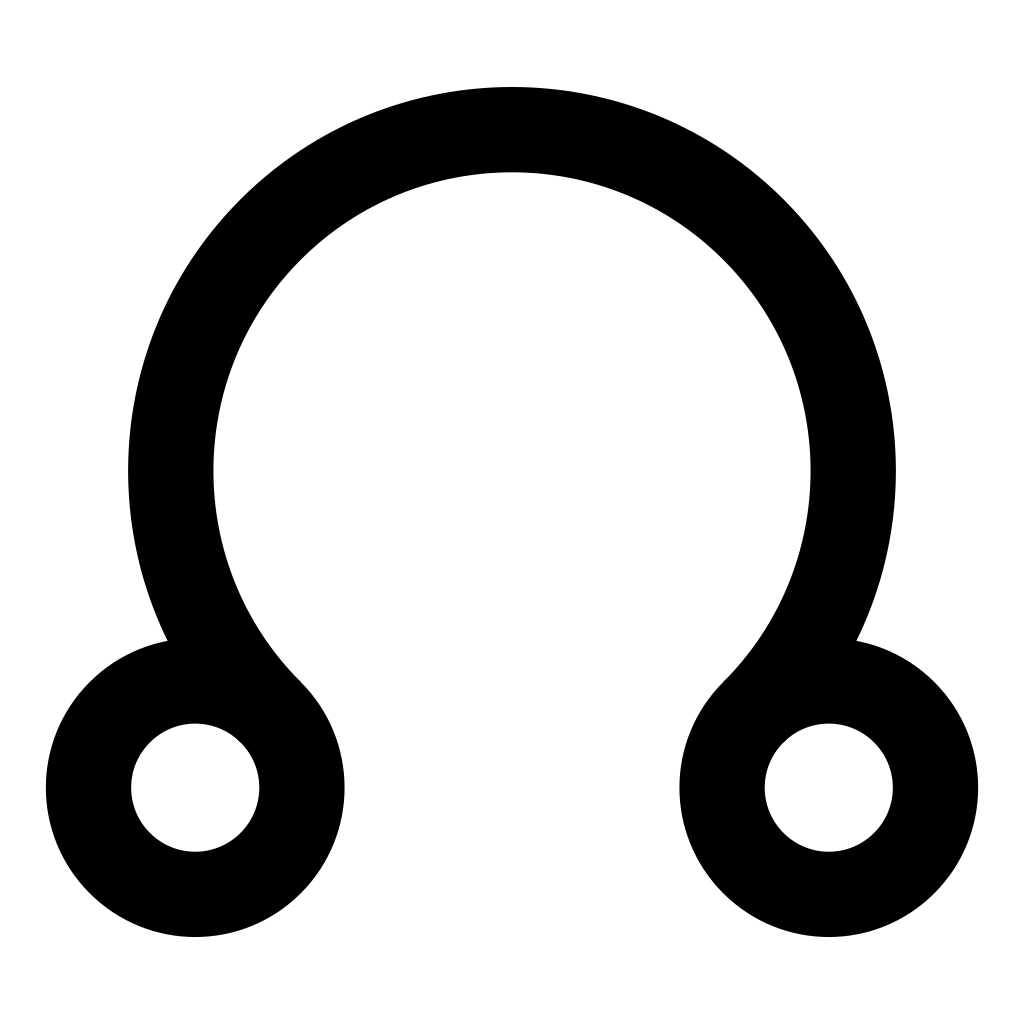
\includegraphics[width=.3cm]{figures/ascending_node}:\\
    point where the orbiting body moves \textbf{north} through the reference plane};
}
\only<5|handout:5>{
    \node[minimum size=\textwidth, align=left, anchor=west] at (-.2, 0) {%
    \begin{varwidth}{\linewidth}
        \begin{description}
            \item[{longitude of the ascending node $\Omega\ [\si{\radian}]$}]\hfill\\\hspace*{-2cm}%
            the angle from the reference direction to the direction of the ascending node; \\\hspace*{-2cm}measured counterclockwise
        \end{description}
    \end{varwidth}};
}
\only<6|handout:6>{
    \node[minimum size=\textwidth, align=left, anchor=west] at (-.2, 0) {%
    \begin{varwidth}{\linewidth}
        \begin{description}
            \item[{argument of periapsis $\omega\ [\si{\radian}]$}]\hfill\\\hspace*{-2cm} 
            angle from the body's ascending node to its periapsis in the direction of motion, e.g.:\\\hspace*{-1cm}
            \begin{tabularx}{.9\textwidth}{rX}
                $\SI{0}{\radian}$ & the orbiting body has its closest approach to the central body at the same moment it crosses the reference frame from south to north 
            \end{tabularx}
        \end{description}
    \end{varwidth}};
}
\only<7|handout:7>{
    \node[minimum size=\textwidth, align=left, anchor=west] at (-.2, 0) {%
    true anomaly $\nu\ [\si{\radian}]$ at epoch $t_0\ [\si{\jd}]$:\\
    angle between the direction of periapsis and the position of the orbiting body at epoch $t_0$};
}
\only<8|handout:8>{
    \node[minimum size=\textwidth, align=left, anchor=west] at (-.2, 0) {%
    \begin{varwidth}{\linewidth}
        \begin{description}
            \item[{mean anomaly $M_0\ [\si{\radian}]$ at epoch $t_0\ [\si{\jd}]$}]\hfill\\\hspace*{-2cm} 
            the angular distance from the pericenter which a fictitious body would have if it \\\hspace*{-2cm}
            moved in a circular orbit, with constant speed, in the same orbital period as the \\\hspace*{-2cm}
            actual body in its elliptical orbit
        \end{description}
    \end{varwidth}};
}
    \end{tikzpicture}
\end{frame}
%%%%%%%%%%%%%%%%%%%%%%%%%%%%%%%%%%%%%%%%%%%%%%%%%%%%%%%%%%%%%%%%%%%%

%%%%%%%%%%%%%%%%%%%%%%%%%%%%%%%%%%%%%%%%%%%%%%%%%%%%%%%%%%%%%%%%%%%%
\begin{frame}
    \frametitle{Orbital Elements - The Six Keplerian Elements (Overview)}
    \hspace{0em}
    \vspace{-1.3em}
    \begin{description}
        \setlength\itemsep{.3em}
        \item[eccentricity $e$]\hfill\\\hspace*{-2cm} 
        shape of the ellipsis (elongation compared to a circle)
        \item[{semi-major axis $a\ [\si{\au}]$}]\hfill\\\hspace*{-2cm} 
        one-half of the largest diameter
        \item[{inclination $i\ [\si{\radian}]$}]\hfill\\\hspace*{-2cm} 
        vertical tilt of the ellipsis with respect to the reference plane
        \item[{longitude of the ascending node $\Omega\ [\si{\radian}]$}]\hfill\\\hspace*{-2cm} 
        the angle from the reference direction to the direction of the ascending node
        \item[{argument of periapsis $\omega\ [\si{\radian}]$}]\hfill\\\hspace*{-2cm}
        angle from the body's ascending node to its periapsis in the direction of motion
        \item[{mean anomaly $M_0\ [\si{\radian}]$ at epoch $t_0\ [\si{\jd}]$}]\hfill\\\hspace*{-2cm} the angular distance from the pericenter which a fictitious body would have if it \\\hspace*{-2cm}
        moved in a circular orbit, with constant speed, in the same orbital period as the \\\hspace*{-2cm}
        actual body in its elliptical orbit
    \end{description}
\end{frame}
%%%%%%%%%%%%%%%%%%%%%%%%%%%%%%%%%%%%%%%%%%%%%%%%%%%%%%%%%%%%%%%%%%%%

%%%%%%%%%%%%%%%%%%%%%%%%%%%%%%%%%%%%%%%%%%%%%%%%%%%%%%%%%%%%%%%%%%%%
\begin{frame}
    \frametitle{Orbital State Vectors - Cartesian Vectors}
    \begin{description}
        \setlength\itemsep{.5em}
        \item[{position $\vec{r}\ [\si{\au}]$}]\hfill\\\hspace*{-2cm} the position of the body in the reference frame, $\vec{r} \in \mathbb{R}^3$
        \item[{velocity $\vec{v}\ [\si{\au\per\day}]$}]\hfill\\\hspace*{-2cm} the velocity of the body in the same reference frame, $\vec{v} \in \mathbb{R}^3$
    \end{description}
\end{frame}
%%%%%%%%%%%%%%%%%%%%%%%%%%%%%%%%%%%%%%%%%%%%%%%%%%%%%%%%%%%%%%%%%%%%

\subsection{Conversion to state vectors}
%%%%%%%%%%%%%%%%%%%%%%%%%%%%%%%%%%%%%%%%%%%%%%%%%%%%%%%%%%%%%%%%%%%%
\begin{frame}
    \frametitle{Convert Orbital Elements to Orbital State Vectors - 1}
    \btVFill
    \begin{enumerate}
        \item Calculate $M(t)$:
        $$ M(t) = M_0 + (t - t_0) \sqrt{\frac{\mu}{a^3}} $$
        where $\mu = GM$ is the standard gravitational parameter of the central body and $t$ the Sun's/Sol's reference epoch at $2451544.5$ JD (midnight on January 1, 2000)\\
        (\textbf{note:} take care of the correct units!).
        \item Solve \textsc{Kepler}'s equation $M(t) = E(t) - e \sin{E(t)}$ for the eccentric anomaly $E(t)$ with a numerical method like \textsc{Newton-Raphson}:
        $$ E_0(t) = M(t) $$
        $$ E_{j+1}(t) = E_j(t) - \frac{E_j(t) - e \sin{E_j(t)} - M(t)}{1 - e \cos{E_j(t)}} $$
        using a suitable stopping criterion (e.g., a fixed number of \num{30} iterations).
    \end{enumerate}
    \btVFill
    \setfontsize{8pt}
    See: \url{https://downloads.rene-schwarz.com/download/M001-Keplerian_Orbit_Elements_to_Cartesian_State_Vectors.pdf}
\end{frame}
%%%%%%%%%%%%%%%%%%%%%%%%%%%%%%%%%%%%%%%%%%%%%%%%%%%%%%%%%%%%%%%%%%%%

%%%%%%%%%%%%%%%%%%%%%%%%%%%%%%%%%%%%%%%%%%%%%%%%%%%%%%%%%%%%%%%%%%%%
\begin{frame}
    \frametitle{Convert Orbital Elements to Orbital State Vectors - 2}
    \btVFill
    \begin{enumerate}
        \setcounter{enumi}{2}
        \item Calculate the true anomaly $\nu(t)$:
        $$ \nu(t) = 2 \cdot\arctan2\left(\sqrt{1 + e} \sin{\frac{E(t)}{2}}, \sqrt{1 - e} \cos{\frac{E(t)}{2}} \right) $$
        \item Calculate the distance to the central body:
        $$ r_c(t) = a(1 - e \cos{E(t)}) $$
        \item Calculate the position $\vec{o}(t)$ and velocity $\dot{\vec{o}}(t)$ vectors in the orbital frame:
        $$ \vec{o}(t) = r_c(t) \begin{pmatrix} \cos{\nu(t)} \\ \sin{\nu(t)} \\ 0 \end{pmatrix}, \quad
           \dot{\vec{o}}(t) = \frac{\sqrt{\mu a}}{r_c(t)} \begin{pmatrix} -\sin{E(t)} \\ \sqrt{1 - e^2} \cos{E(t)} \\ 0 \end{pmatrix} $$
    \end{enumerate}
    \btVFill
    \setfontsize{8pt}
    See: \url{https://downloads.rene-schwarz.com/download/M001-Keplerian_Orbit_Elements_to_Cartesian_State_Vectors.pdf}
\end{frame}
%%%%%%%%%%%%%%%%%%%%%%%%%%%%%%%%%%%%%%%%%%%%%%%%%%%%%%%%%%%%%%%%%%%%

%%%%%%%%%%%%%%%%%%%%%%%%%%%%%%%%%%%%%%%%%%%%%%%%%%%%%%%%%%%%%%%%%%%%
\begin{frame}
    \frametitle{Convert Orbital Elements to Orbital State Vectors - 3}
    \btVFill
    \begin{enumerate}
        \setcounter{enumi}{5}
        \item Transform $\vec{o}(t)$ and $\dot{\vec{o}}(t)$ to the inertial frame in bodycentric rectangular coordinates $\vec{r}(t)$ and $\dot{\vec{r}}(t)$ using the matrix $R$:
        $$R = \begin{pmatrix} 
                \cos{\omega}\cos{\Omega} - \sin{\omega}\cos{i}\sin{\Omega} & -(\sin{\omega}\cos{\Omega} + \cos{\omega}\cos{i}\sin{\Omega}) & 0 \\ 
                \cos{\omega}\sin{\Omega} + \sin{\omega}\cos{i}\cos{\Omega} & \cos{\omega}\cos{i}\cos{\Omega} - \sin{\omega}\sin{\Omega} & 0 \\ 
                \sin{\omega}\sin{i} & \cos{\omega}\sin{i} & 0
              \end{pmatrix}$$
        $$ \vec{r}(t) = R \cdot \vec{o}(t), \quad 
           \dot{\vec{r}}(t) = R \cdot \dot{\vec{o}}(t)$$
        % \item Convert $\vec{r}(t)$ and $\dot{\vec{r}}(t)$ to the respective output units $\si{\au}$ and $\si{\au\per\day}$:
        % $$ \vec{r}(t)_{[\si{\au}]} = \vec{r}(t) \cdot \frac{\num{1}}{\num{1.49597870691e11}}, $$
        % $$ \dot{\vec{r}}(t)_{[\si{\au\per\day}]} = \dot{\vec{r}}(t) \cdot \frac{\num{86400}}{\num{1.49597870691e11}} $$
        \item Update position and velocity to be relative to its central body $cb$:
        $$ \vec{r}(t) = \vec{r}(t) + \vec{r}_{cb}(t), \quad
           \dot{\vec{r}}(t) = \dot{\vec{r}}(t) + \dot{\vec{r}}_{cb}(t)$$
    \end{enumerate}
    \btVFill
    \setfontsize{8pt}
    See: \url{https://downloads.rene-schwarz.com/download/M001-Keplerian_Orbit_Elements_to_Cartesian_State_Vectors.pdf}
\end{frame}
%%%%%%%%%%%%%%%%%%%%%%%%%%%%%%%%%%%%%%%%%%%%%%%%%%%%%%%%%%%%%%%%%%%%